\section{网络模型结构}
\subsection*{网络模型结构}
\frame{
	\frametitle{网络整体结构}
	\begin{figure}[h]
		\centering
		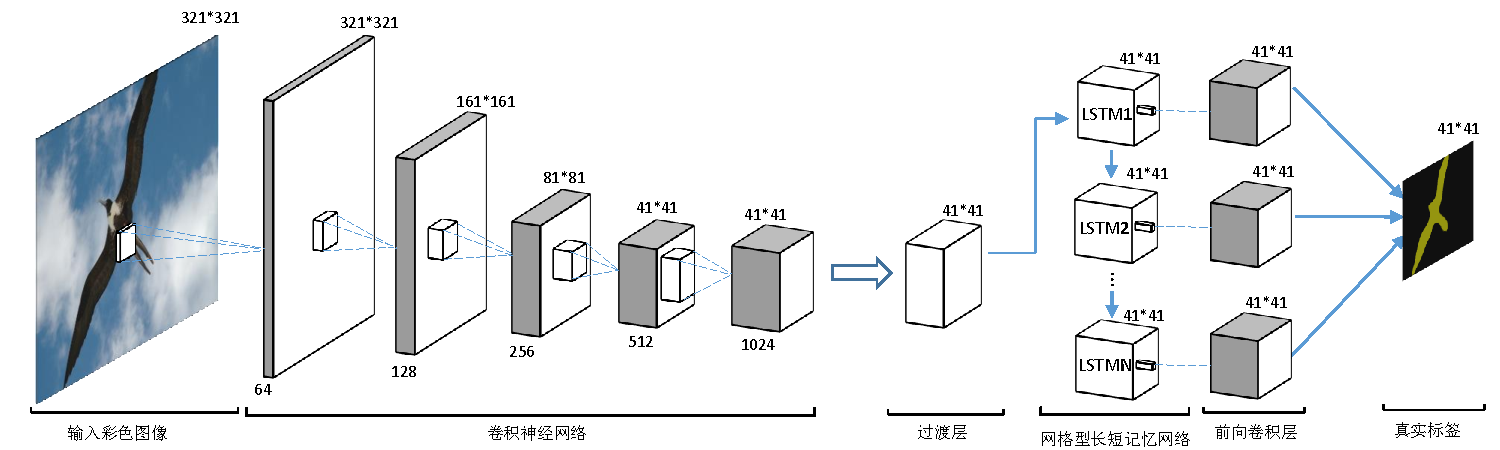
\includegraphics[width=0.9\textwidth,height=0.28\textwidth]{image/chap04/illustration/networkstructure.pdf}
		\caption{网络整体结构图}
		\label{fig:networkstructure}
	\end{figure}
	\vspace{-1em}
	\small
	\begin{block}{}
		\begin{itemize}
			\item  四个组成部分:\textbf{卷积网络部分},过渡层,\textbf{网格型长短记忆网络部分},前向卷积层
			\item 核心思想:在卷积网络后堆叠多层网格型长短记忆层
		\end{itemize}
	\end{block}
}
\frame{
	\frametitle{卷积网络部分}
	\vspace{-1em}
	\footnotesize
	\begin{block}{}
		\begin{itemize}
			\item 基于$VGG_{16}$模型\footnote{Simonyan \& Zissermanet, Very deep Convolutional Networks For Large-scale Image Recognition, ICLR 2015}, 含有16层卷积层
			\item 使用了“孔算法”,在不损失精度的情况下将模型参数减少了 6.5 倍\footnote{Chen et al, DeepLab-LargeFOV, ICLR 2015}
		\end{itemize}
	\end{block}
	\vspace{-1em}
	\begin{figure}[h]
		\centering
		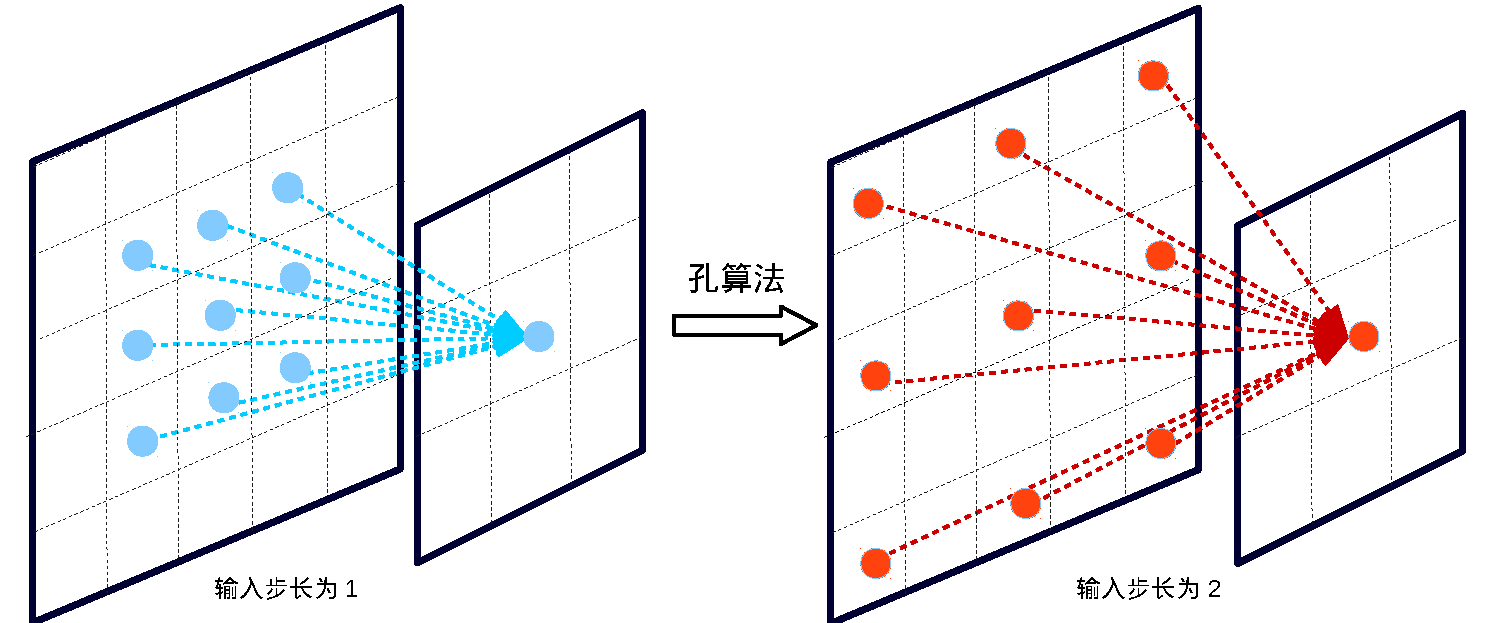
\includegraphics[width=0.7\textwidth]{image/chap04/illustration/hole.pdf}
		\caption{"孔算法"示意图}
	\end{figure}
}

\frame{
	\frametitle{网格型长短记忆网络部分}
	\vspace{-1em}
	\begin{columns}%[onlytextwidth]
		\begin{column}{0.6\textwidth}
			\vspace{0.2em}
			\begin{figure}
				\centering
				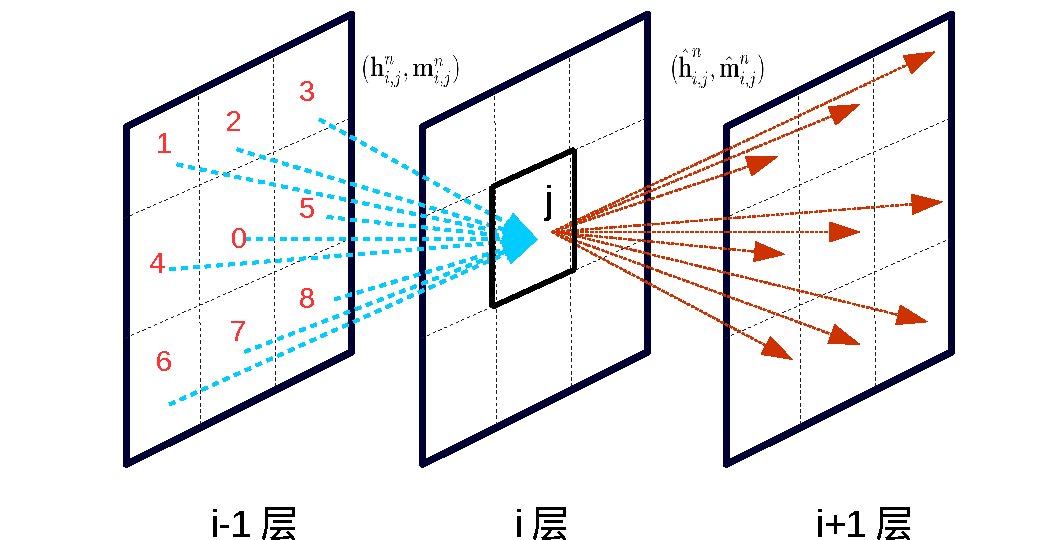
\includegraphics[width=\textwidth]{image/chap04/illustration/neighboring.pdf}
				\caption{九维网格型长短记忆网络层之间的通信示意图}
				\label{fig:neighboring}
			\end{figure}
		\end{column}
		%%%%%%% new column
		\begin{column}{0.5\textwidth}
			\footnotesize
			\vspace{-1.5em}
			\begin{align}
				\begin{split}
					(\hat{\textbf{h}}_{i,j}^0,\hat{\textbf{m}}_{i,j}^0) &= \mbox{LSTM}(\textbf{H}_{i,j},\textbf{m}_{i,j}^0,\textbf{W}_i) \\
					(\hat{\textbf{h}}_{i,j}^1,\hat{\textbf{m}}_{i,j}^1) &= \mbox{LSTM}(\textbf{H}_{i,j},\textbf{m}_{i,j}^1,\textbf{W}_i) \\
					\vdots \\
					(\hat{\textbf{h}}_{i,j}^N,\hat{\textbf{m}}_{i,j}^N) &= \mbox{LSTM}(\textbf{H}_{i,j},\textbf{m}_{i,j}^N,\textbf{W}_i) \\
					\textbf{H}_{i,j} &= [\textbf{h}_{i,j}^0\mbox{ }\textbf{h}_{i,j}^1\mbox{ }...\mbox{ }\textbf{h}_{i,j}^N]^T
				\end{split}
			\end{align}
		\end{column}
	\end{columns}
	\footnotesize
	\vspace{-1em}
	\begin{block}{九维网格型长短记忆网络}
		\vspace{-0.7em}
		\begin{itemize}
			\item 每个位置的预测会受到上一层相邻八邻域特征的影响
			\item 随着层数的堆叠,每一位置将会有更大的感知域。
			\item 网格型长短记忆网络的层数通过实验来确定
		\end{itemize}
	\end{block}
}


